\documentclass[tikz,border=8pt]{standalone}
\usepackage[utf8]{inputenc}
\usepackage{amsmath,amssymb}
\usepackage{microtype}
\usetikzlibrary{arrows.meta,calc,positioning}

\definecolor{maroon}{RGB}{122,36,53}
\definecolor{taupe}{RGB}{124,95,88}
\definecolor{gold}{RGB}{154,106,31}
\definecolor{muted}{RGB}{124,116,104}
\definecolor{rule}{RGB}{189,169,132}

\begin{document}
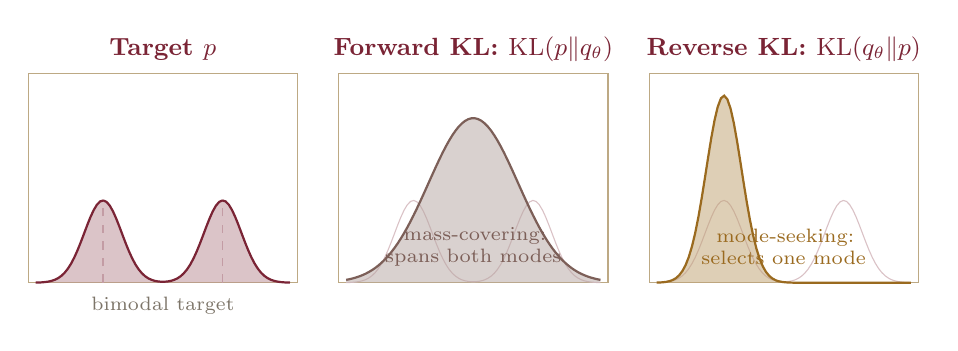
\begin{tikzpicture}[font=\small,scale=0.95]
\def\pw{3.6}
\def\ph{2.8}
\def\gap{0.55}

% Target distribution
\begin{scope}[shift={(0,0)}]
  \node[font=\small\bfseries,maroon] at (\pw/2,\ph+0.32)
    {Target $p$};
  \draw[rule] (0,0) rectangle (\pw,\ph);
  \fill[maroon!52,opacity=0.52,domain=0.1:3.5,samples=80,variable=\x]
    plot(\x,{2.0*(0.55*exp(-8*(\x-1.0)*(\x-1.0))
                    +0.55*exp(-8*(\x-2.6)*(\x-2.6)))})
    -- (3.5,0) -- (0.1,0) -- cycle;
  \draw[maroon,thick,domain=0.1:3.5,samples=80]
    plot(\x,{2.0*(0.55*exp(-8*(\x-1.0)*(\x-1.0))
                    +0.55*exp(-8*(\x-2.6)*(\x-2.6))) });
  \draw[maroon!45,dashed,thin] (1.0,0) -- (1.0,1.12);
  \draw[maroon!45,dashed,thin] (2.6,0) -- (2.6,1.12);
  \node[muted,font=\scriptsize] at (\pw/2,-0.3) {bimodal target};
\end{scope}

% Forward KL approximation
\begin{scope}[shift={(\pw+\gap,0)}]
  \node[font=\small\bfseries,maroon] at (\pw/2,\ph+0.32)
    {Forward KL: $\mathrm{KL}(p\|q_\theta)$};
  \draw[rule] (0,0) rectangle (\pw,\ph);
  \draw[maroon!28,thin,domain=0.1:3.5,samples=80]
    plot(\x,{2.0*(0.55*exp(-8*(\x-1.0)*(\x-1.0))
                    +0.55*exp(-8*(\x-2.6)*(\x-2.6))) });
  \fill[taupe!55,opacity=0.52,domain=0.1:3.5,samples=80,variable=\x]
    plot(\x,{2.2*exp(-1.4*(\x-1.8)*(\x-1.8))})
    -- (3.5,0) -- (0.1,0) -- cycle;
  \draw[taupe,thick,domain=0.1:3.5,samples=80]
    plot(\x,{2.2*exp(-1.4*(\x-1.8)*(\x-1.8))});
  \node[taupe,font=\scriptsize,align=center,text width=2.8cm]
    at (\pw/2,0.48) {mass-covering:\\spans both modes};
\end{scope}

% Reverse KL approximation
\begin{scope}[shift={(2*\pw+2*\gap,0)}]
  \node[font=\small\bfseries,maroon] at (\pw/2,\ph+0.32)
    {Reverse KL: $\mathrm{KL}(q_\theta\|p)$};
  \draw[rule] (0,0) rectangle (\pw,\ph);
  \draw[maroon!28,thin,domain=0.1:3.5,samples=80]
    plot(\x,{2.0*(0.55*exp(-8*(\x-1.0)*(\x-1.0))
                    +0.55*exp(-8*(\x-2.6)*(\x-2.6))) });
  \fill[gold!62,opacity=0.52,domain=0.1:3.5,samples=80,variable=\x]
    plot(\x,{2.5*exp(-9.0*(\x-1.0)*(\x-1.0))})
    -- (3.5,0) -- (0.1,0) -- cycle;
  \draw[gold,thick,domain=0.1:3.5,samples=80]
    plot(\x,{2.5*exp(-9.0*(\x-1.0)*(\x-1.0))});
  \node[gold,font=\scriptsize,align=center,text width=2.8cm]
    at (\pw/2,0.48) {mode-seeking:\\selects one mode};
\end{scope}
\end{tikzpicture}
\end{document}
